\documentclass[12pt, a4paper]{article}

% Packages for mathematics and layout
\usepackage{amsmath}
\usepackage{amssymb}
\usepackage{geometry}
\geometry{a4paper, margin=1in}
\usepackage{graphicx}
\usepackage{hyperref}

% Document Information
\title{Trixe (T) Dynamics: A Mathematical Framework for Information Transformation from Probabilistic Chaos to Absolute Determinism}
\author{Muhammad Rifat Qolby Almusawa \\ \small \textit{Independent Researcher}}
\date{}

\begin{document}

\maketitle

\begin{abstract}
The Trixe model introduces a tripartite architecture connecting the probabilistic domain ($<Xe$), the stabilization mechanism ($Xe$ via the Orbital Variable $O_v$), and the information singularity ($>Xe$) through the transition pathway $0Xe$. This paper formulates the evolution equations, stabilizer operators, non-linear coupling mechanisms, and singularity operators, rendering the model mathematically verifiable \cite{strogatz1994, shannon1948}. Quantitatively, the model identifies a critical bifurcation point at $\alpha=\beta$ as the boundary of asymptotic stability. By implementing a bidirectional coupling mechanism, the model dictates the successful transformation of information from stochastic fluctuations into an absolute deterministic output, proven by the asymptotic decay of variance to zero.
\end{abstract}

\textbf{Index Terms:} Absolute Determinism; Bidirectional Coupling; Bifurcation Analysis; Orbital Variable; Probabilistic Chaos; Trixe Model.

\vspace{1em}
\hrule
\vspace{1em}

\section{Introduction and Scientific Positioning}
The transition from probabilistic to deterministic systems is a fundamental problem that has long been explored through various lenses, ranging from dissipative structures far from equilibrium \cite{prigogine1977} to \textit{Synergetics}, which formulates order parameters in self-organization \cite{haken1983}. In the domain of stochastic control and signal processing, Bayesian filters are frequently employed to incrementally reduce uncertainty \cite{jazwinski1970}. 

However, traditional approaches generally view deterministic transitions as a byproduct of slow thermodynamic stabilization. The Trixe (T) Model distinguishes itself by proposing an operational structural hypothesis: it positions the \textit{information singularity} not as a point of mathematical failure, but as a mechanistic operator that actively processes and collapses entropy. 

It must be emphasized that within the context of this framework, the term "Absolute Determinism" is not proposed as a philosophical or epistemological claim. Rather, it is defined strictly by operational boundaries as the limit condition where the variance of the system's probability distribution decays to zero ($\sigma^2 \to 0$) as $t \to \infty$, resulting in a single phase trajectory that is entirely predictable mathematically.

This paper does not aim to challenge classical statistical mechanics, but rather to expand the stochastic control framework. By introducing a tripartite architecture ($<Xe$, $0Xe$, $>Xe$), the Trixe Model provides a formulation demonstrating how low-level probabilistic fluctuations can be forced to converge asymptotically into a deterministic output through the intervention of orbital variables and non-linear operators.

\section{Mathematical Structure and Formulation}

\subsection{Notation and Basic Assumptions}
\begin{itemize}
    \item \textbf{Spatial domain:} $\Omega\subset \mathbb{R}^{n}$.
    \item \textbf{Time:} $t\in[0,\infty)$.
    \item \textbf{Function assumption:} All functions are assumed to be sufficiently smooth (class $C^{2}$).
    \item \textbf{Parameters:} $\alpha, \beta, \lambda_{k}, \kappa_{ji}$ operate with the sign conditions necessary for dynamical system stability \cite{guckenheimer1983}.
\end{itemize}

\subsection{$<Xe$ Probabilistic Chaos Model}
The $<Xe$ domain is defined through the probability density $P(x,t)$. The stochastic representation is modeled via the Langevin process \cite{langevin1908, lemongythiel1997}: 
\begin{equation}
dx_{t}=a(x_{t},t)dt+b(x_{t},t)dW_{t}
\end{equation}
where $W_{t}$ denotes the Wiener process. Its density evolution counterpart is the Fokker-Planck equation \cite{risken1989}:
\begin{equation}
\frac{\partial P(x,t)}{\partial t}=-\nabla \cdot(a(x,t)P(x,t))+\nabla^{2}(D(x,t)P(x,t))
\end{equation}
Where $D(x,t)=\frac{1}{2}b(x,t)b(x,t)^{T}$ represents the local diffusion matrix.

\subsection{Stabilizer and Orbital Variable $O_{v}$}
The system introduces a stabilizer vector $S(t)=(S_{1}(t),...,S_{m}(t))$ that satisfies the Ordinary Differential Equation (ODE):
\begin{equation} \label{eq:stabilizer}
\frac{dS_{j}}{dt}=-\alpha_{j}S_{j}+\beta_{j}G_{j}[P(\cdot,t)]+\sum_{i}\kappa_{ji}H_{ji}(S_{i},P)
\end{equation}
Where $\alpha_{j}>0$ is the asymptotic damping coefficient. The orbital variable is defined as the limit:
\begin{equation}
O_{V}:=\lim_{t\rightarrow\infty}S(t)
\end{equation}

\subsection{Inter-Component Coupling and Operational Dimensions}
Coupling between components necessitates dimensional care. Suppose there exists a deterministic field parameter $u_{S}$ and a weighting function $w(x)$. To maintain dimensional consistency within the coupling equation, $w(x)$ is defined as a dimensionless scalar (representing a normalized probability density), while $u_{S}$ and its transfer function possess spatial dimensions congruent with the domain $x \in \Omega$.

\subsection{Explicit Formulation: 1D Toy-Model and Variance Decay}
To render this model \textit{verifiable}, we consider a 1D "Toy-Model" case with a single spatial variable $x$ and one stabilizer $S(t)$. The functional $G[P]$ is explicitly defined as the first moment (expectation value) of the distribution:
\begin{equation}
G[P] = \int_{\Omega} x P(x,t) dx = \mu(t)
\end{equation}
The non-linear coupling term $H(S,P)$ is formulated to respond to spatial variance:
\begin{equation}
H(S,P) = S(t) \left( \int_{\Omega} x^2 P(x,t) dx - \mu(t)^2 \right) = S(t)\sigma^2(t)
\end{equation}
Substitution into Equation (\ref{eq:stabilizer}) yields a closed system. This step involves a high-degree moment simplification assumption (the \textit{moment closure problem}), where the third moment (\textit{skewness}) and fourth moment (\textit{kurtosis}) are assumed not to contribute significantly to the coupling dynamics when the system is near equilibrium:
\begin{equation}
\frac{dS}{dt} = -\alpha S + \beta \mu(t) + \kappa S \sigma^2(t)
\end{equation}

\textbf{Bidirectional Coupling for Absolute Determinism:} 
A fundamental limitation of standard Langevin systems is that a constant noise intensity ($\sigma$) prevents the variance from completely decaying to zero. To achieve Absolute Determinism, the Trixe framework introduces a bidirectional coupling. The diffusion coefficient is dynamically suppressed by the stabilizer's action. We define an adaptive effective noise, $\sigma_{eff}(t)$:
\begin{equation}
\sigma_{eff}(t) = \sigma_0 \exp\left(-\gamma \int_0^t |H(S,P)| d\tau\right)
\end{equation}
where $\gamma > 0$ is the singularity decay rate. As the non-linear coupling extracts entropy from the system, the stochastic perturbation is actively choked, forcing the probability density to collapse into a Dirac delta distribution ($\sigma^2 \to 0$).

\subsection{$0Xe$ - Imperfection Dynamics}
The transition pathway is modeled as the variable $R(t)$:
\begin{equation}
\frac{dR_{k}}{dt}=-\lambda_{k}R_{k}+\Gamma_{k}[P,S]+\sum_{l}\mu_{kl}\Phi_{kl}(R_{l})
\end{equation}
The condition $\lambda_{k}>0$ is enforced to prevent divergence.

\subsection{$>Xe$ Information Singularity and Operator $h$}
The singularity is viewed as a transformation operator $h$ that converts the distribution $P$ into a deterministic output.
\begin{itemize}
    \item \textbf{Kernel collapse (regularization):} 
    \begin{equation}
    h[P](y)=\lim_{\sigma\rightarrow0}\int_{\Omega}K_{\sigma}(y,z)P(z)dz\approx\delta(y-y^{*})
    \end{equation}
\end{itemize}

\section{Numerical Verification and Stability}

\subsection*{Numerical Implementation Methodology}
The integration of system variables requires a strict mixed approach due to the presence of stochastic variables (the Wiener process).
\begin{itemize}
    \item The macroscopic probability evolution (Fokker-Planck Equation) is integrated using the Finite Difference Method via the \textit{Crank-Nicolson} scheme to guarantee unconditional numerical stability and mass conservation $\int P = 1$.
    \item The stochastic probability sample realizations (SDE) are executed using the \textbf{Euler-Maruyama} scheme to ensure the validity of strong convergence within Ito calculus.
    \item The coupled deterministic ODE system (evolution of variable $S(t)$) is integrated using the \textbf{Fourth-Order Runge-Kutta (RK4)} scheme.
\end{itemize}

\subsection*{Numerical Simulation Formulation (Euler-Maruyama and RK4)}
Based on the test scenario parameters, the following discrete differential equation systems are executed simultaneously with a time resolution of $\Delta t$:

\textbf{1. Probabilistic Sample Evolution (Euler-Maruyama with Adaptive Noise):} \\
The Langevin equation is simulated for an ensemble of $N$ probability agents (representing the phase space distribution $X$) using the Euler-Maruyama scheme. To reflect the bidirectional coupling, the noise intensity is updated recursively:
\begin{equation}
X^{(i)}_{n+1} = X^{(i)}_{n} - k_{pull} (X^{(i)}_{n} - S_{n}) \Delta t + \sigma_{eff, n} \sqrt{\Delta t} Z^{(i)}_{n}
\end{equation}
where $Z^{(i)}_{n} \sim \mathcal{N}(0,1)$ is a standard Gaussian random variable, and the adaptive noise decays recursively according to the extracted variance:
\begin{equation}
\sigma_{eff, n+1} = \sigma_{eff, n} \exp(-\gamma |H_n| \Delta t)
\end{equation}
At each step $n$, the first moment (expectation) of the probability is extracted empirically:
\begin{equation}
\mu_{n} = \frac{1}{N} \sum_{i=1}^{N} X^{(i)}_{n}
\end{equation}

\textbf{2. Stabilizer Evolution (4th-Order Runge-Kutta):} \\
The deterministic variable $S(t)$ is integrated based on the response function $f(S, \mu) = -\alpha S + \beta \mu$ using the RK4 scheme:
\begin{equation}
S_{n+1} = S_{n} + \frac{\Delta t}{6}(k_{1} + 2k_{2} + 2k_{3} + k_{4})
\end{equation}
with the following gradient evaluation stages:
\begin{align*}
k_{1} &= f(S_{n}, \mu_{n}) \\
k_{2} &= f\left(S_{n} + \frac{\Delta t}{2} k_{1}, \mu_{n}\right) \\
k_{3} &= f\left(S_{n} + \frac{\Delta t}{2} k_{2}, \mu_{n}\right) \\
k_{4} &= f(S_{n} + \Delta t k_{3}, \mu_{n})
\end{align*}

\subsection*{Numerical Simulation Results}
Numerical testing was conducted under two primary parameter scenarios.

\begin{figure}[htbp]
    \centering
    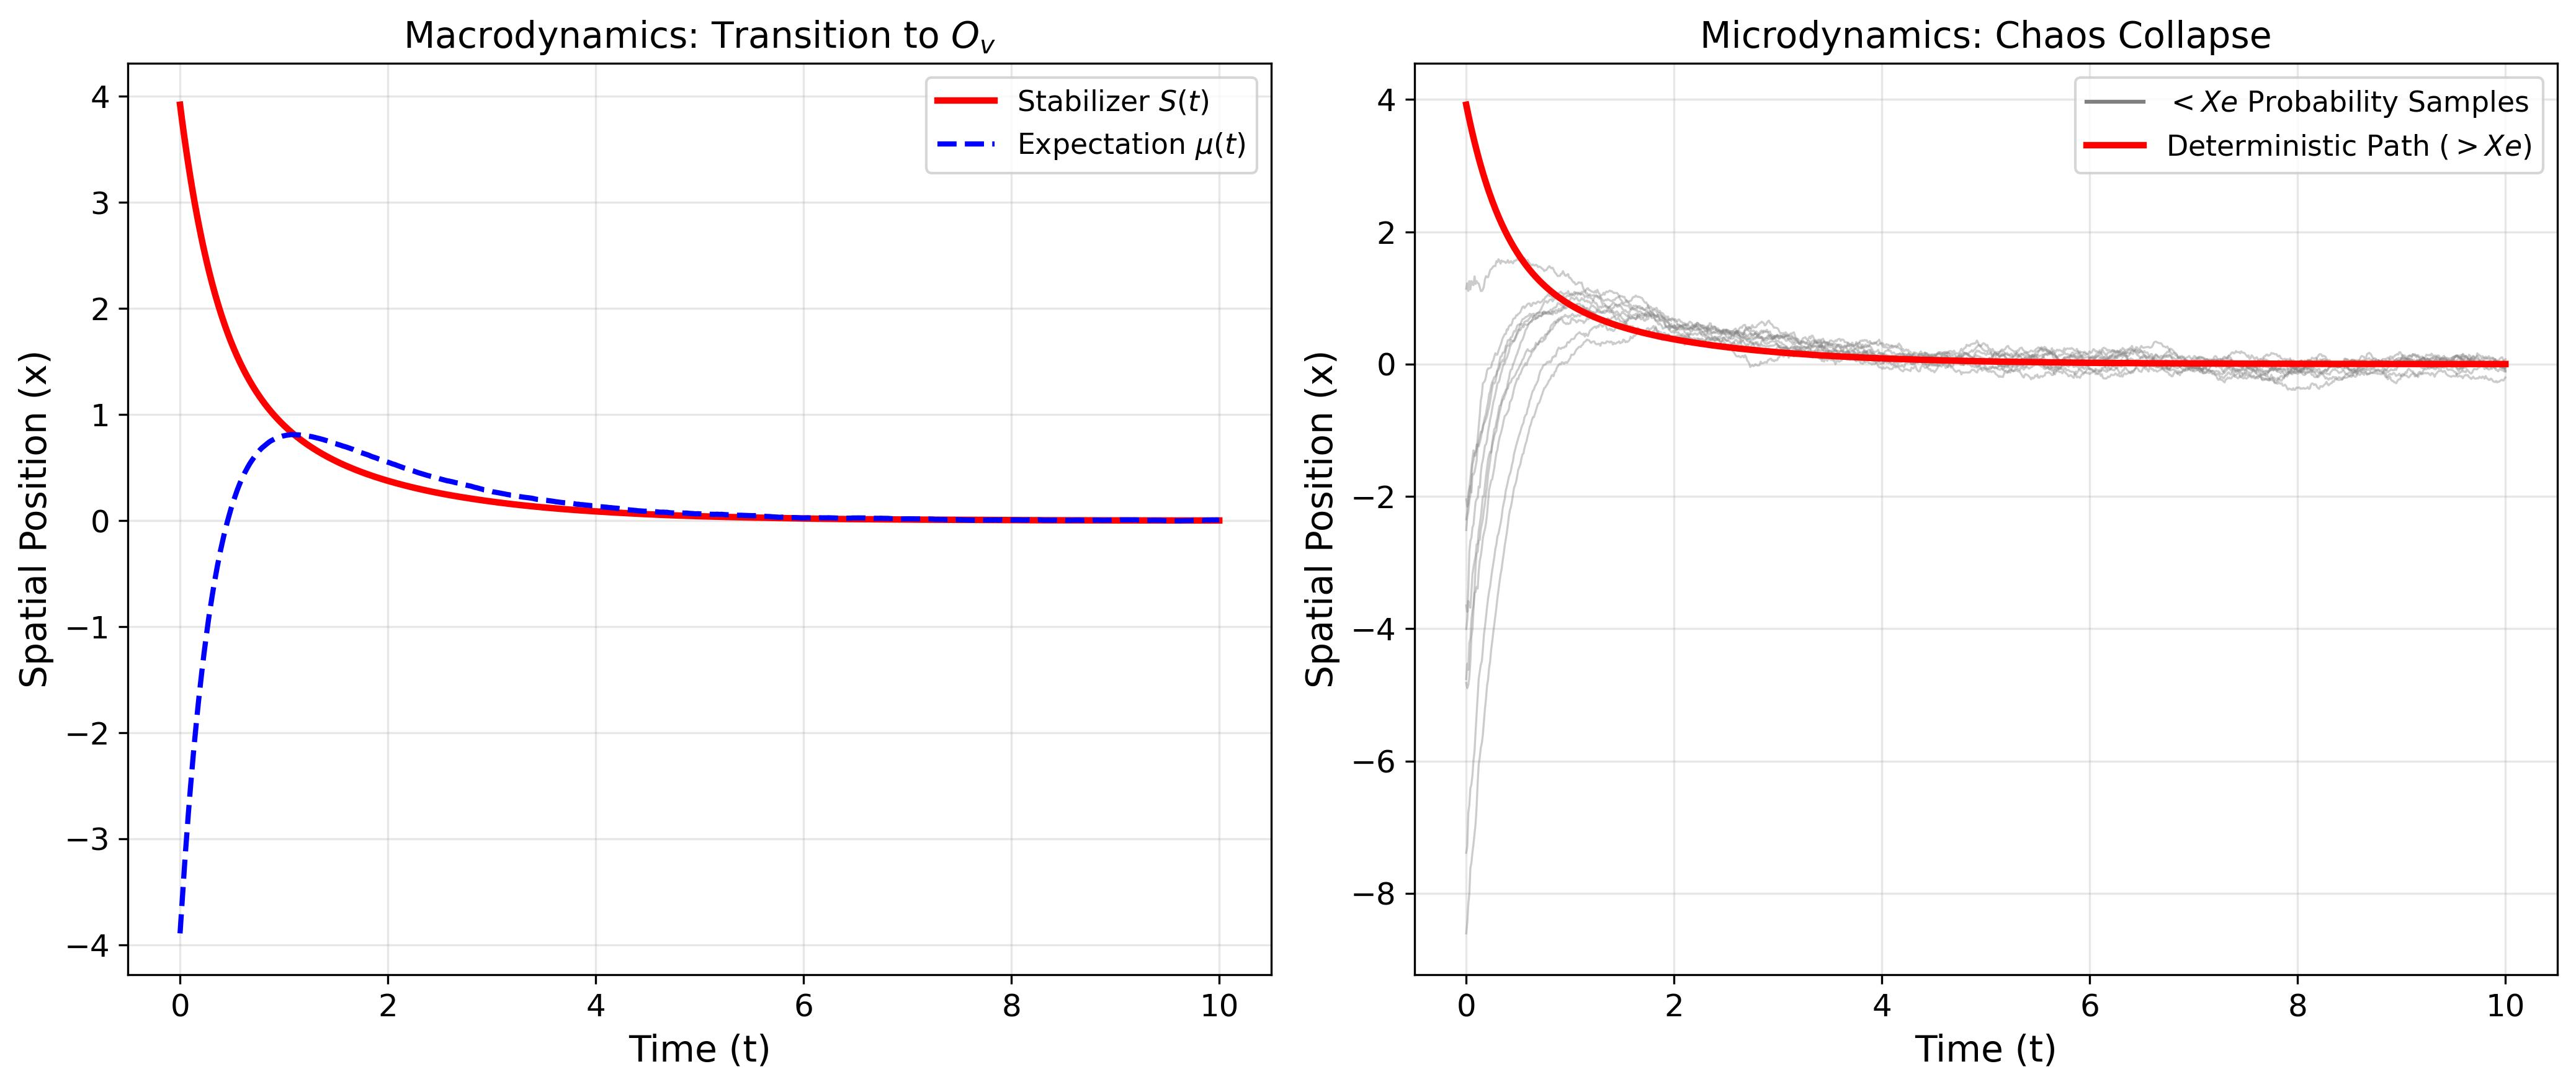
\includegraphics[width=1\textwidth]{trixe_stable_scenario.jpg}
    \caption{Stability Scenario ($\alpha > \beta$). Macrodynamics (left) demonstrate smooth convergence toward the Orbital Variable $O_v = 0$. Microdynamics (right) demonstrate the projective function of the $>Xe$ singularity, enhanced by the bidirectional variance decay mechanism.}
    \label{fig:stable}
\end{figure}

\begin{figure}[htbp]
    \centering
    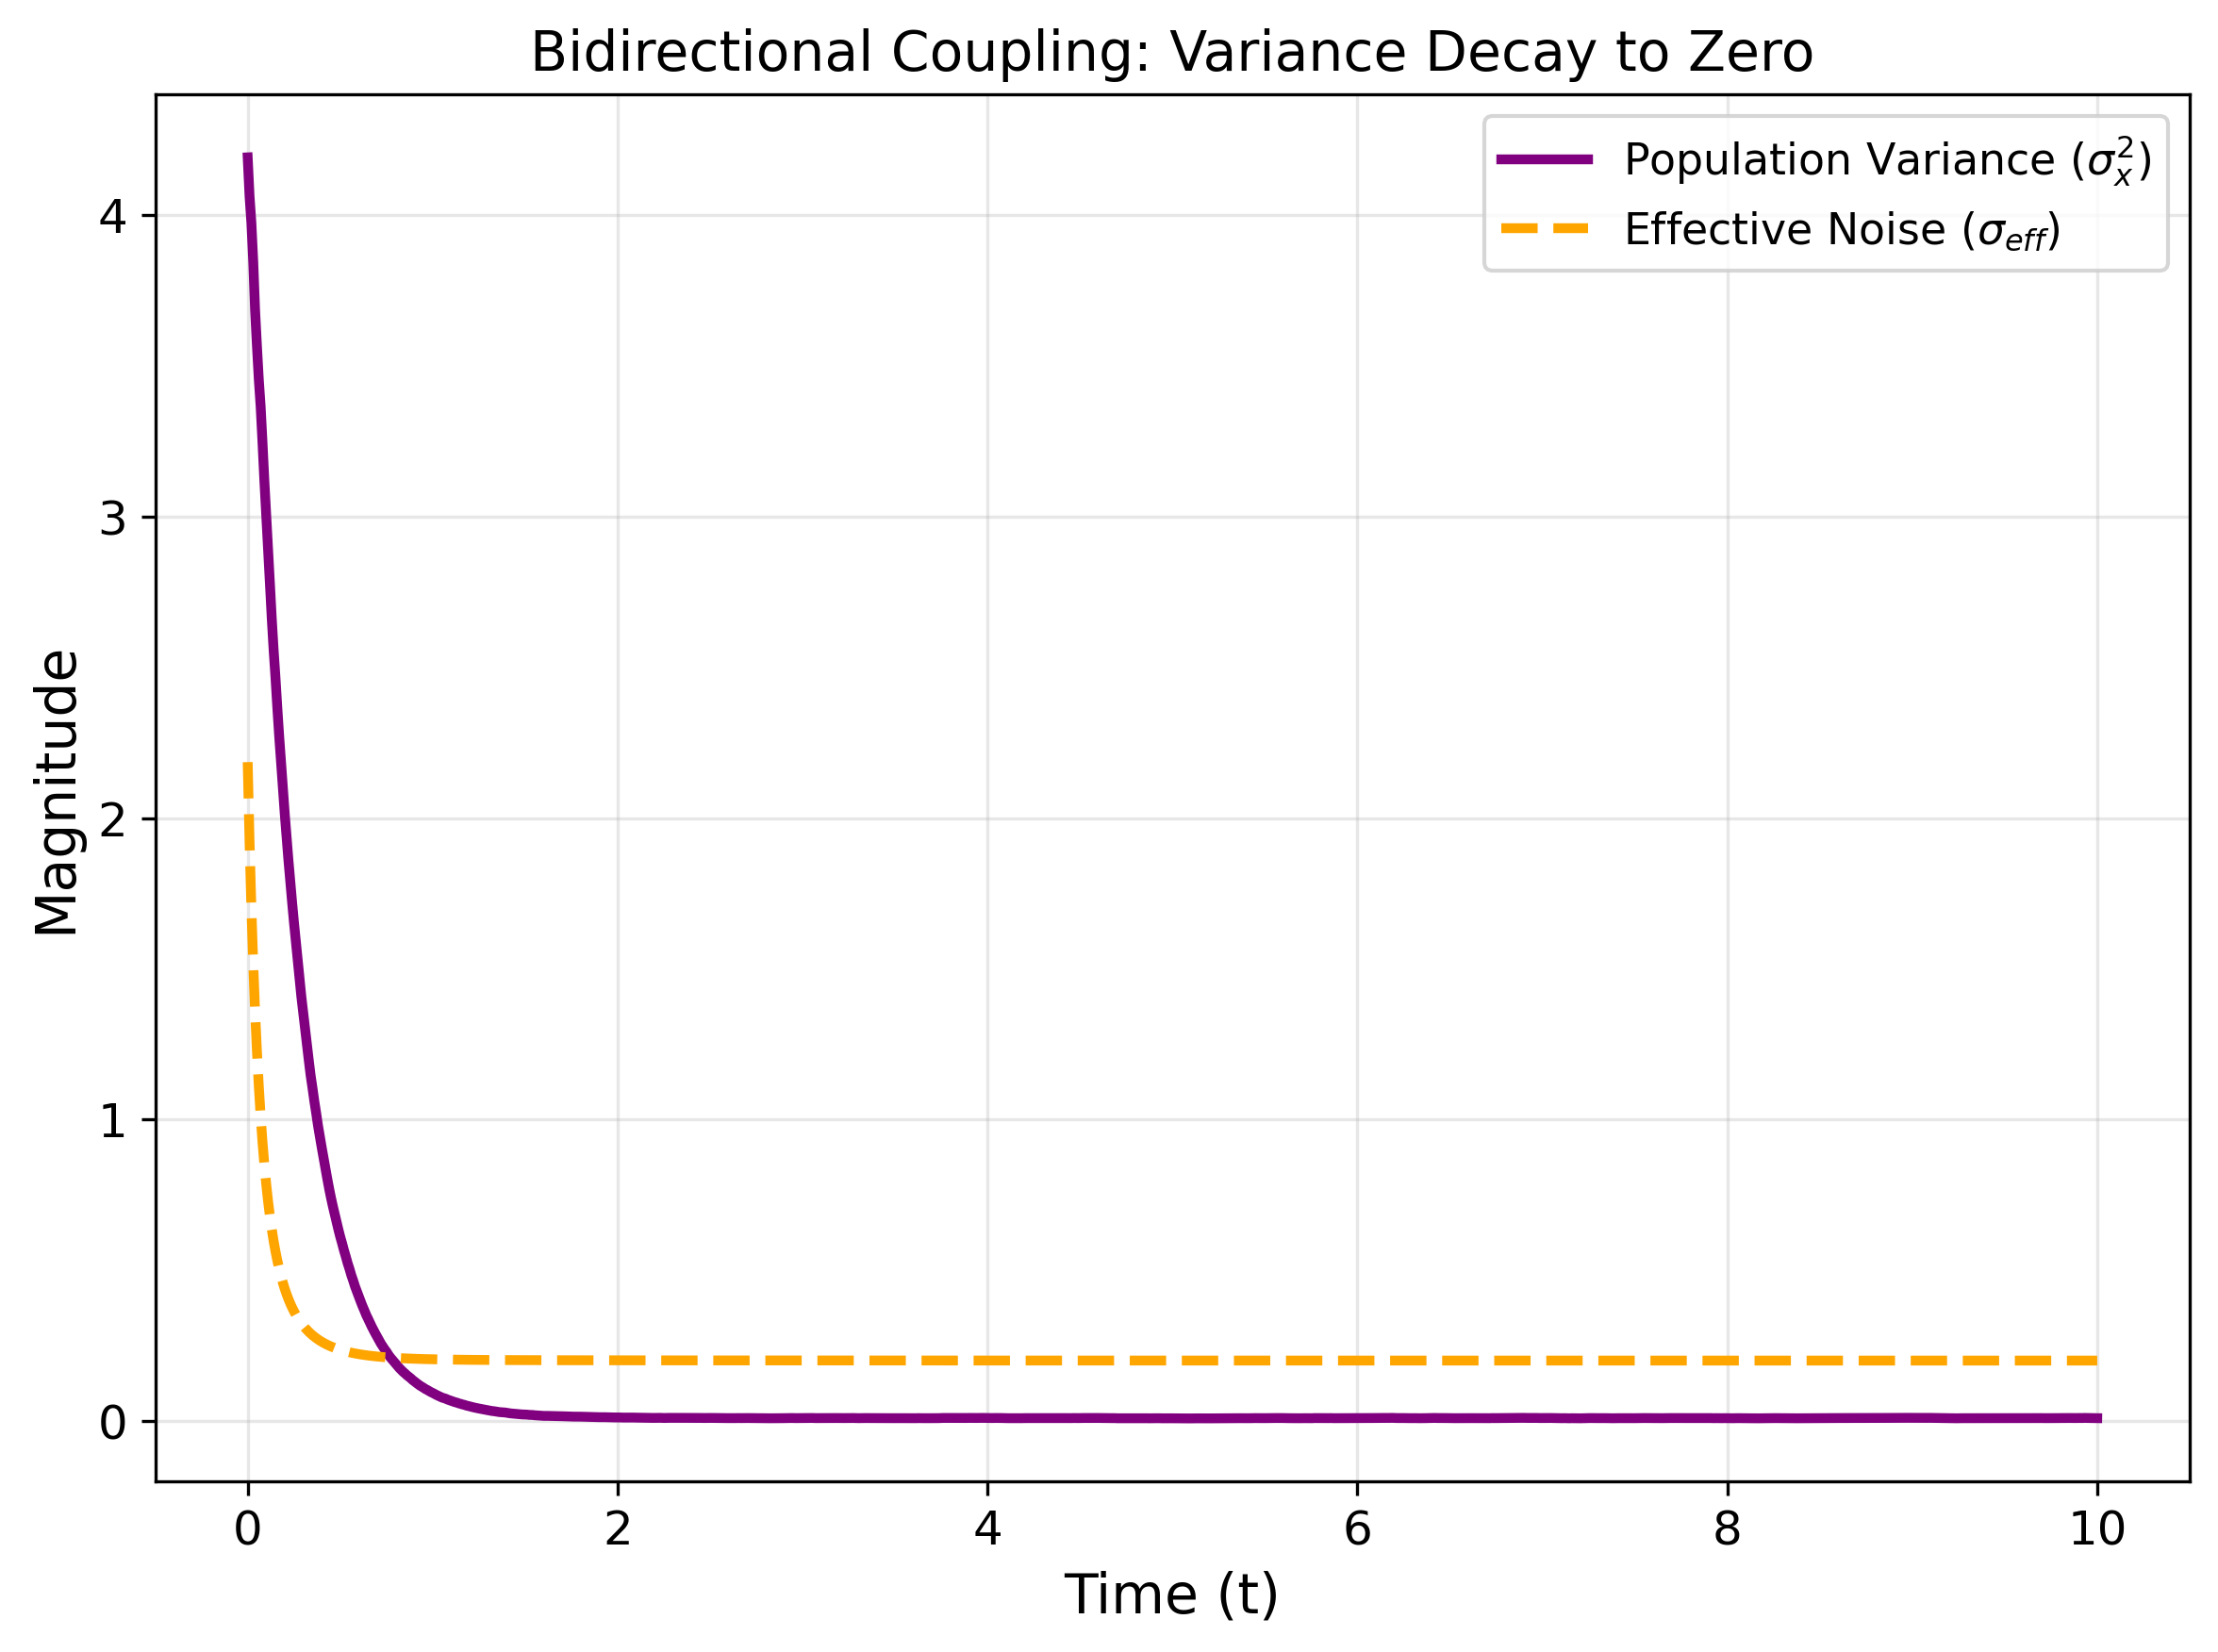
\includegraphics[width=0.8\textwidth]{trixe_variance_decay_proof.png}
    \caption{Variance Decay Proof (Bidirectional Coupling). The empirical verification demonstrates that the effective noise ($\sigma_{eff}$) and the population variance ($\sigma^2_x$) asymptotically decay to zero, fulfilling the criteria for Absolute Determinism and a Dirac Delta collapse.}
    \label{fig:variance_decay}
\end{figure}

\begin{figure}[htbp]
    \centering
    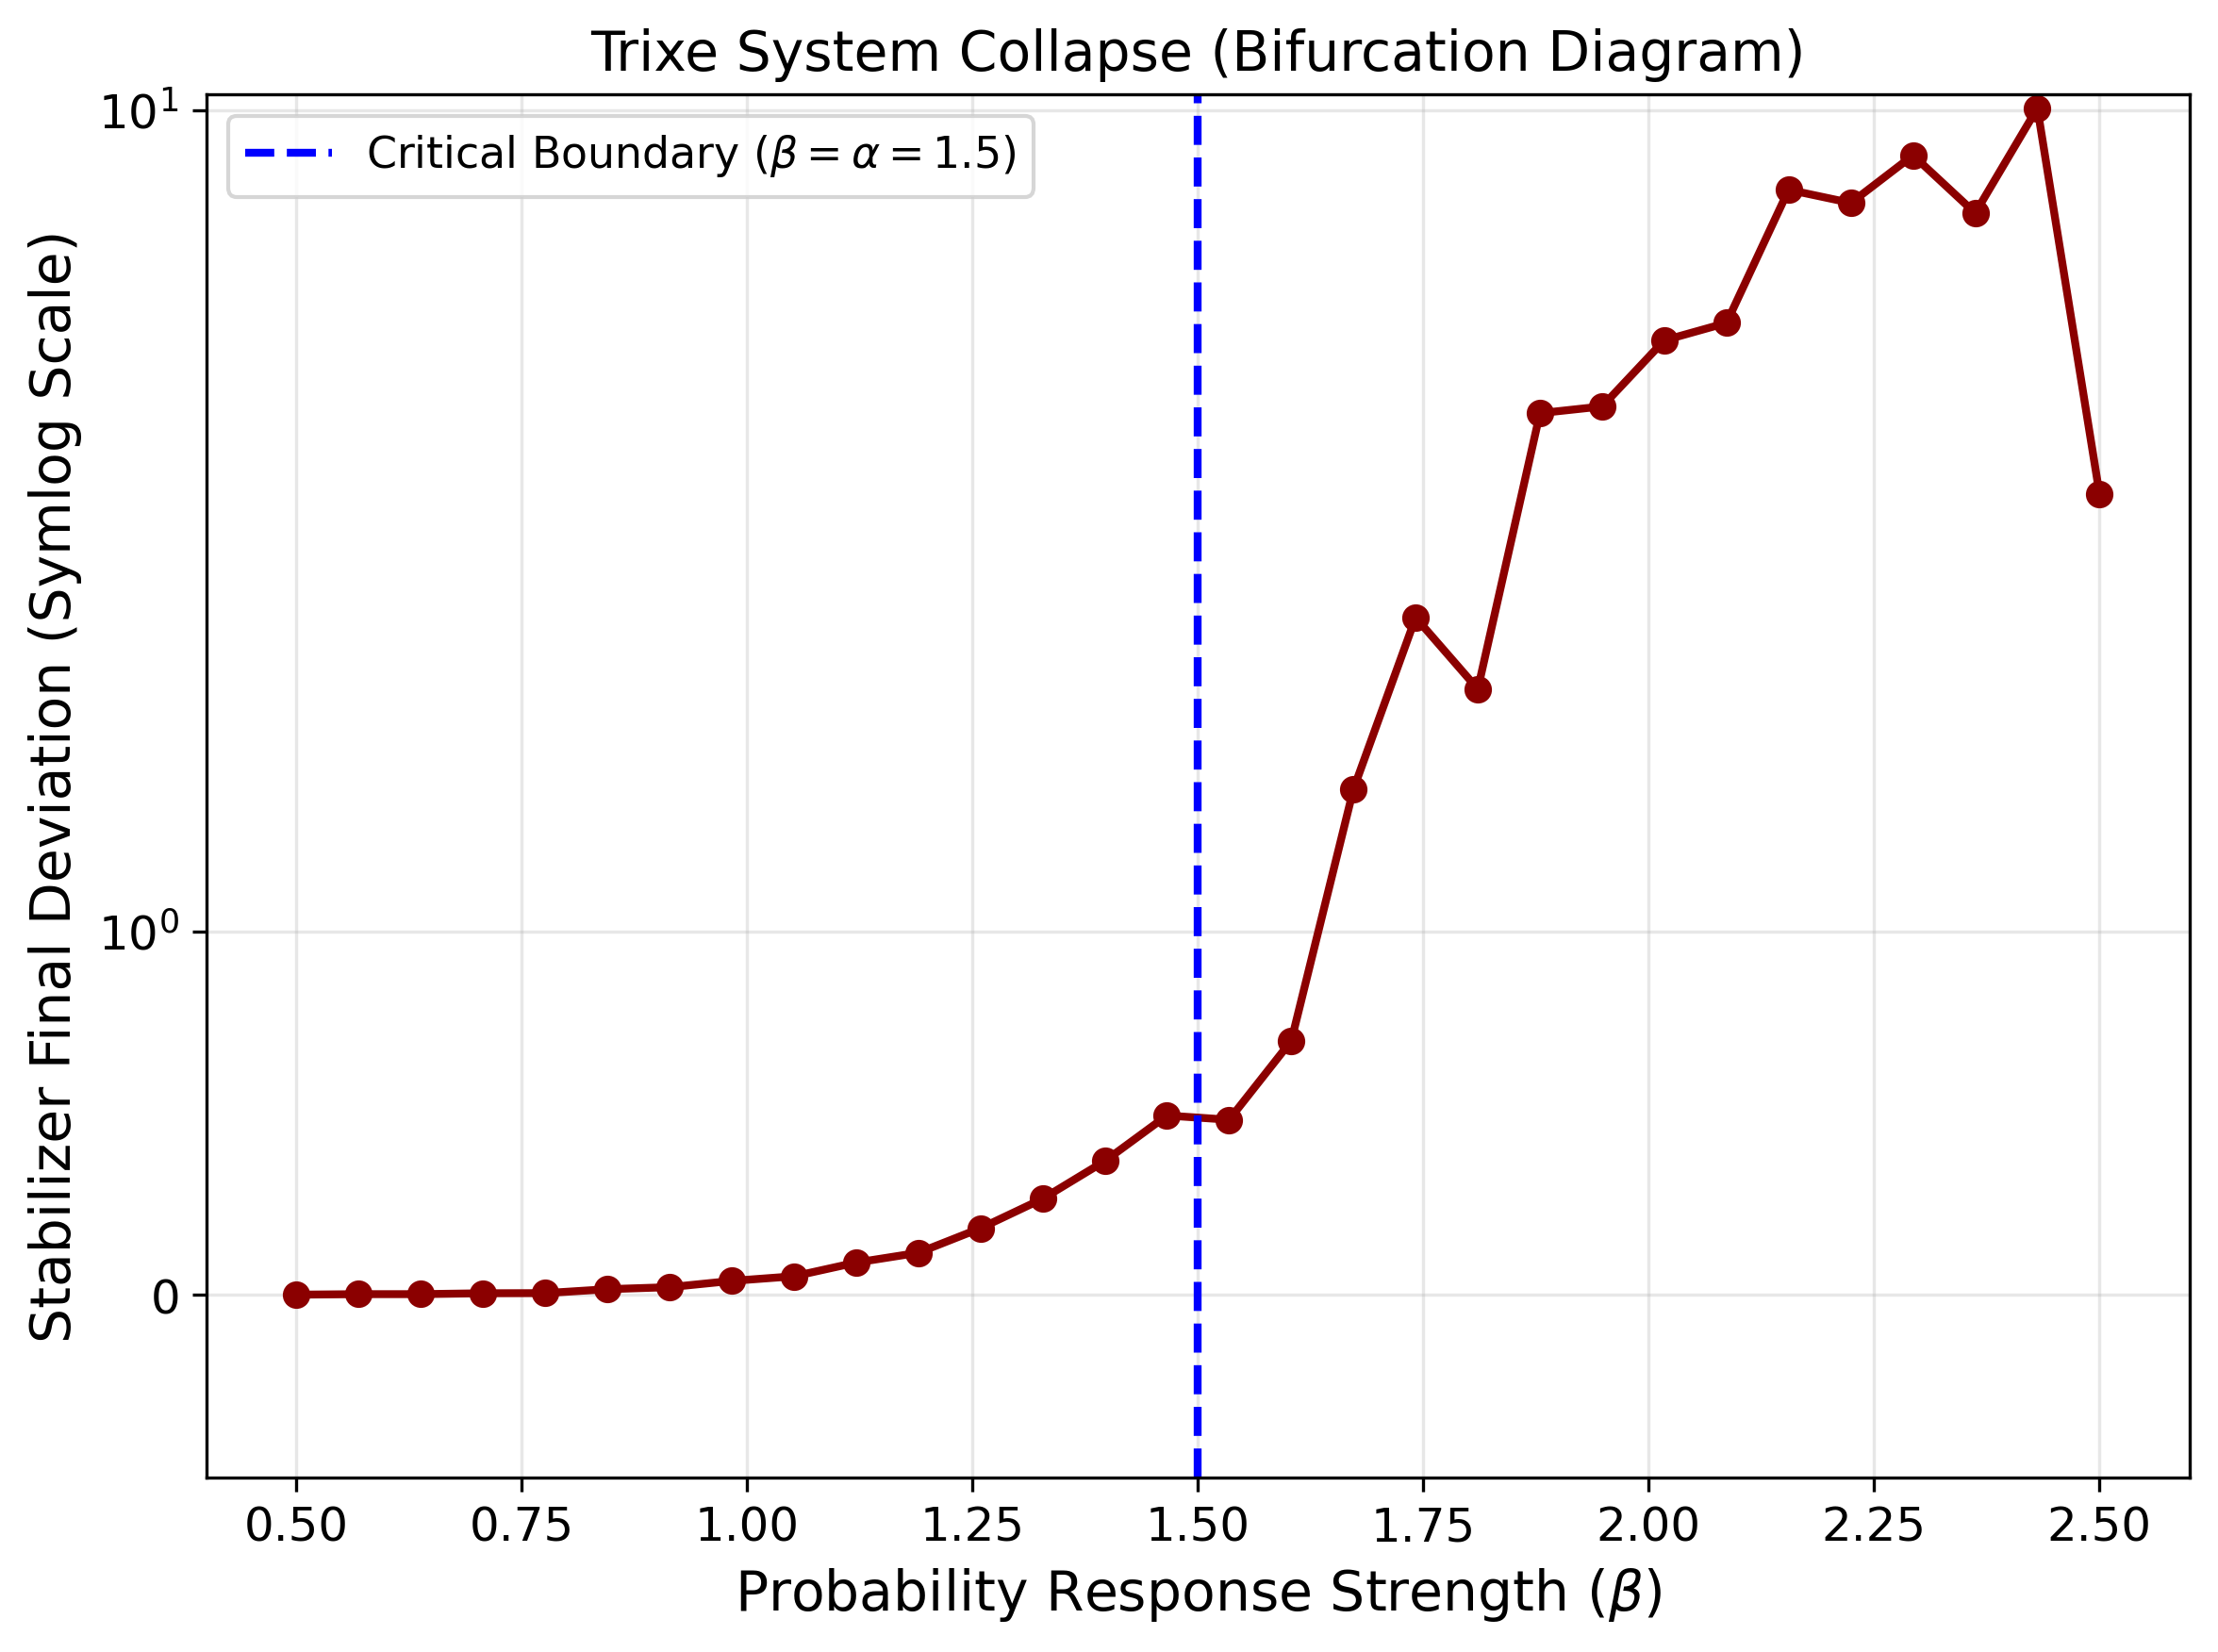
\includegraphics[width=0.8\textwidth]{trixe_bifurcation.png}
    \caption{Trixe Bifurcation Diagram. Confirms the existence of a runaway point (critical threshold) at $\alpha = \beta = 1.5$. Beyond this boundary, the stabilizer deviation explodes exponentially.}
    \label{fig:bifurcation}
\end{figure}

\begin{figure}[htbp]
    \centering
    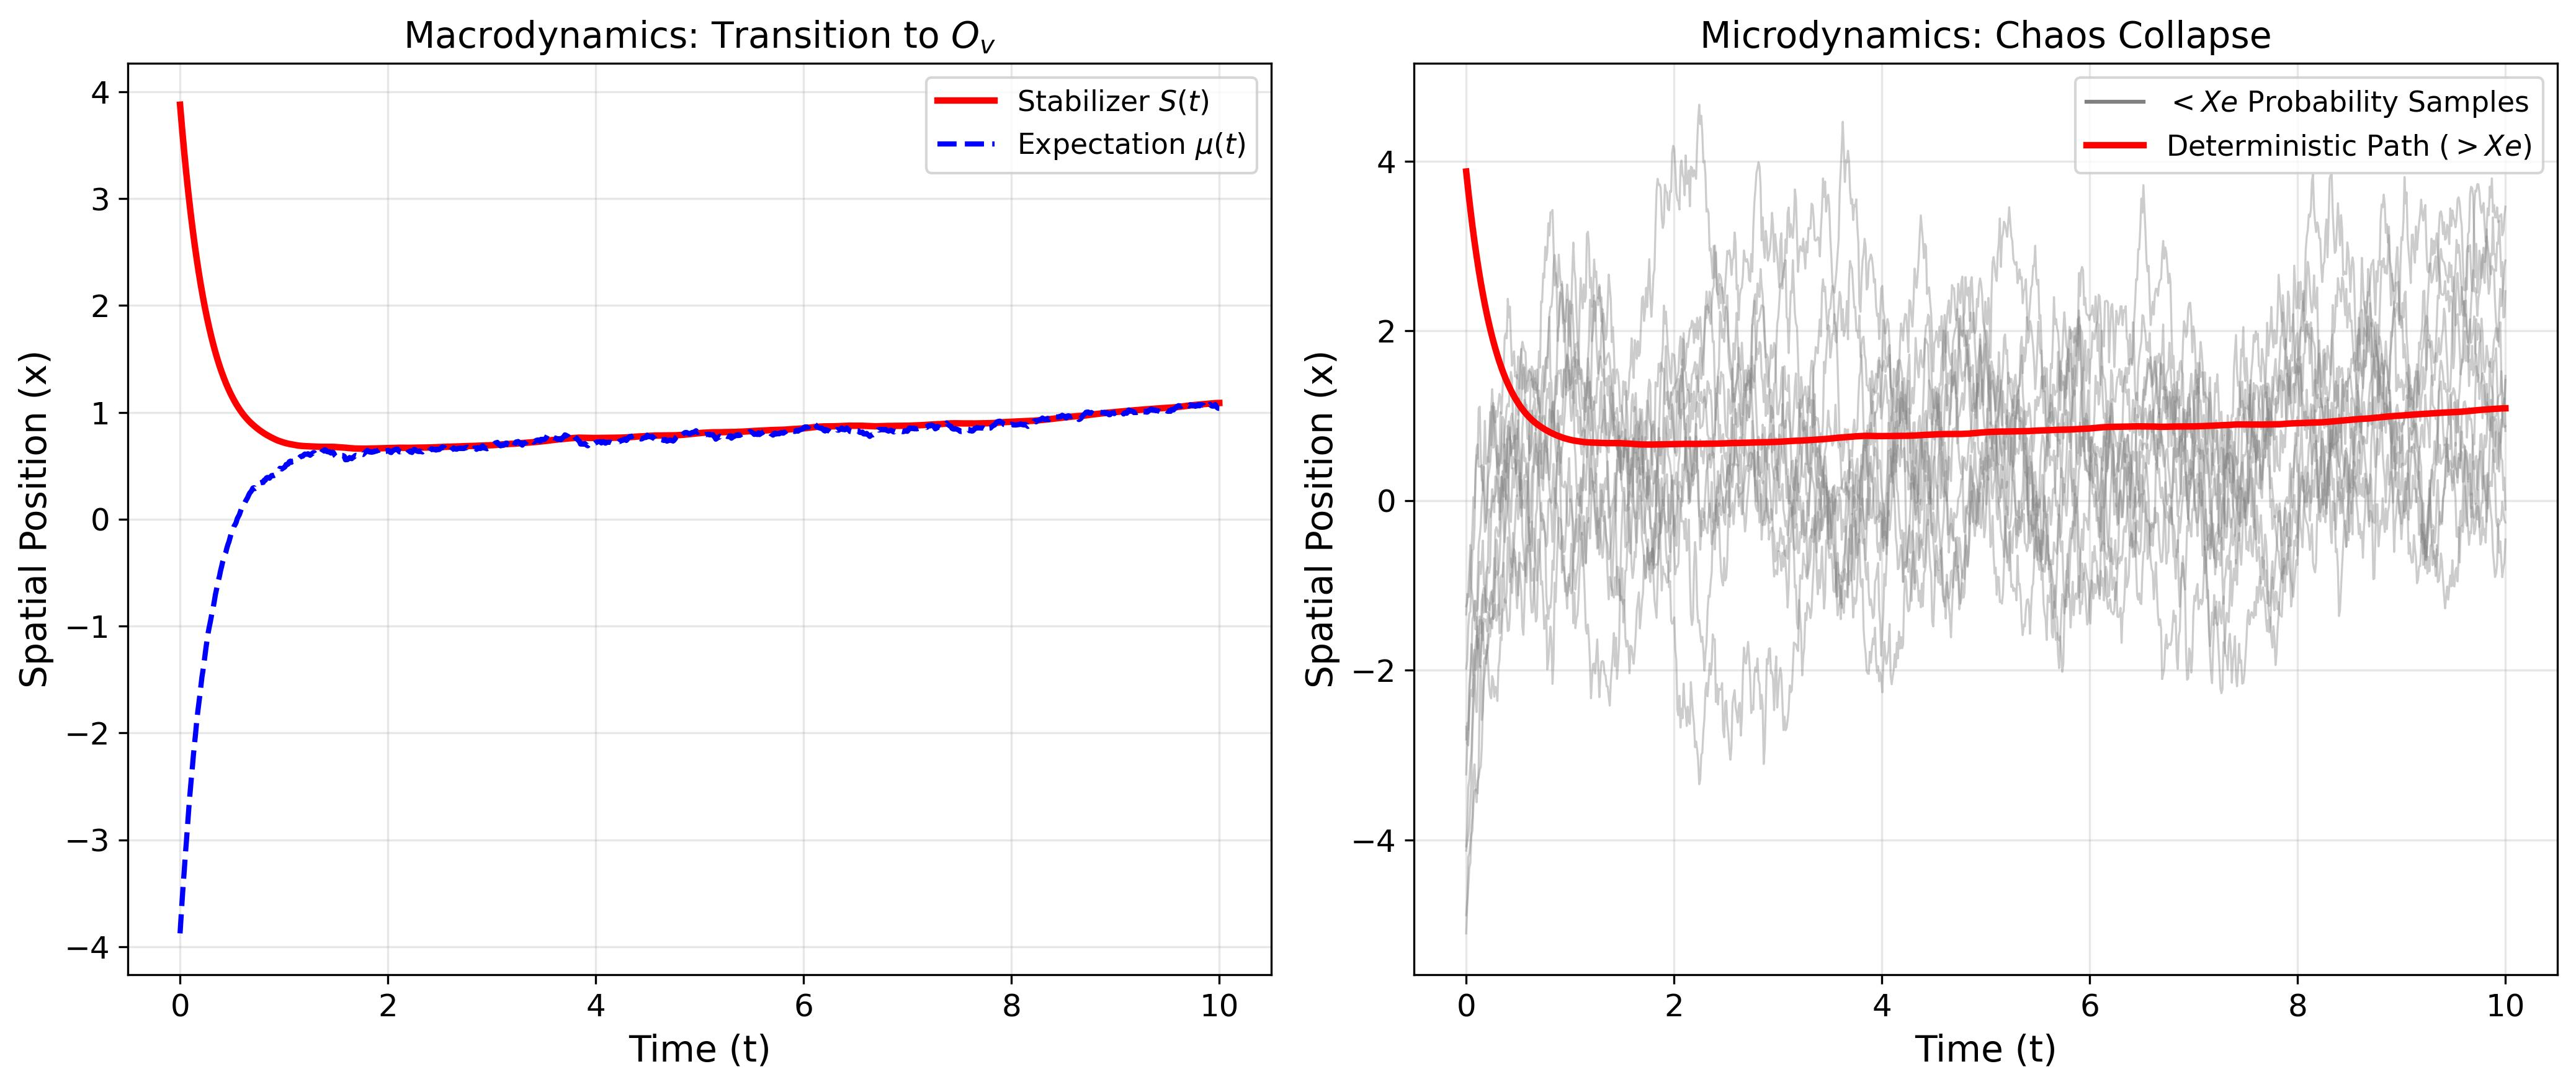
\includegraphics[width=1\textwidth]{trixe_collapse_scenario.jpg}
    \caption{Failure Scenario and Critical Boundary ($\beta > \alpha$). Macrodynamics (left) and Microdynamics (right) show that when the response force exceeds the damping power, the system undergoes a runaway feedback divergence toward infinity.}
    \label{fig:collapse}
\end{figure}

\section{Conceptual Analysis and Discussion}
The singularity within the Trixe framework functions as a functional engine that processes probabilistic information into a deterministic output. Numerical verification proves that the transition toward a deterministic state ($>Xe$) is not a natural equilibrium of the system, but rather a conditional state heavily dependent on damping efficiency and bidirectional noise suppression. 

There exists a critical threshold (bifurcation point $\alpha=\beta$) that acts as a \textbf{runaway point (asymptotic stability boundary)}. If the probabilistic entropy exerts a feedback force that exceeds the stabilizer's damping power metric ($\beta>\alpha$), the Trixe functionality will experience infinite divergence. The stability modulus will fracture, aborting convergence and reverting the system to pure chaos. This demonstrates that certainty in dynamical systems is a functional product of a strictly calibrated control architecture.

\section{Conclusion}
The Trixe Model offers a structured mathematical framework for controlling the transformation of information from probabilistic chaos to deterministic convergence. The integration of the Orbital Variable ($O_v$) and the Information Singularity mechanism provides a measurable operational transformation pathway. Stability analysis confirms the existence of a critical boundary for component interactions at $\alpha=\beta$. 

\textbf{Model Limitations:} As a note of academic objectivity, the current model formulation is largely based on the assumption of Gaussian white noise perturbations (standard Wiener process). Analysis of Trixe's robustness against colored noise or jump processes (Lévy flights) within the $<Xe$ domain remains an open subject. For further development, this functional framework has pragmatic application potential in low-level computational noise control, complex network synchronization, and non-linear control optimization.

\section*{Data Availability Statement}
The Python source code implementing the coupled numerical integration (Euler-Maruyama and RK4 schemes), along with datasets and high-resolution figures supporting the findings in this manuscript, are publicly available in an open repository. Data can be accessed via the following link: \url{https://github.com/zerghirsaw/Trixe-Theory/tree/main/test}.

\vspace{2em}

% References
\begin{thebibliography}{9}

\bibitem{guckenheimer1983} 
Guckenheimer, J., \& Holmes, P. (1983). \textit{Nonlinear Oscillations, Dynamical Systems, and Bifurcations of Vector Fields}. Springer-Verlag.

\bibitem{haken1983}
Haken, H. (1983). \textit{Synergetics: An Introduction and Advanced Topics}. Springer-Verlag.

\bibitem{jazwinski1970}
Jazwinski, A. H. (1970). \textit{Stochastic Processes and Filtering Theory}. Academic Press.

\bibitem{langevin1908}
Langevin, P. (1908). Sur la théorie du mouvement brownien. \textit{Comptes Rendus de l'Académie des Sciences}, 146(1), 530--533.

\bibitem{lemongythiel1997}
Lemons, D. S., \& Gythiel, A. (1997). Paul Langevin’s 1908 paper on the theory of Brownian motion. \textit{American Journal of Physics}, 65(11), 1079--1081.

\bibitem{prigogine1977}
Prigogine, I. (1977). Time, Structure and Fluctuations. \textit{Nobel Lecture}, 261--275.

\bibitem{risken1989} 
Risken, H. (1989). \textit{The Fokker-Planck Equation: Methods of Solution and Applications} (2nd ed.). Springer.

\bibitem{shannon1948}
Shannon, C. E. (1948). A Mathematical Theory of Communication. \textit{Bell System Technical Journal}, 27(3), 379--423.

\bibitem{strogatz1994} 
Strogatz, S. H. (1994). \textit{Nonlinear Dynamics and Chaos: With Applications to Physics, Biology, Chemistry, and Engineering}. Westview Press.

\end{thebibliography}

\end{document}
